% Created by tikzDevice version 0.10.1 on 2018-01-31 10:27:37
% !TEX encoding = UTF-8 Unicode
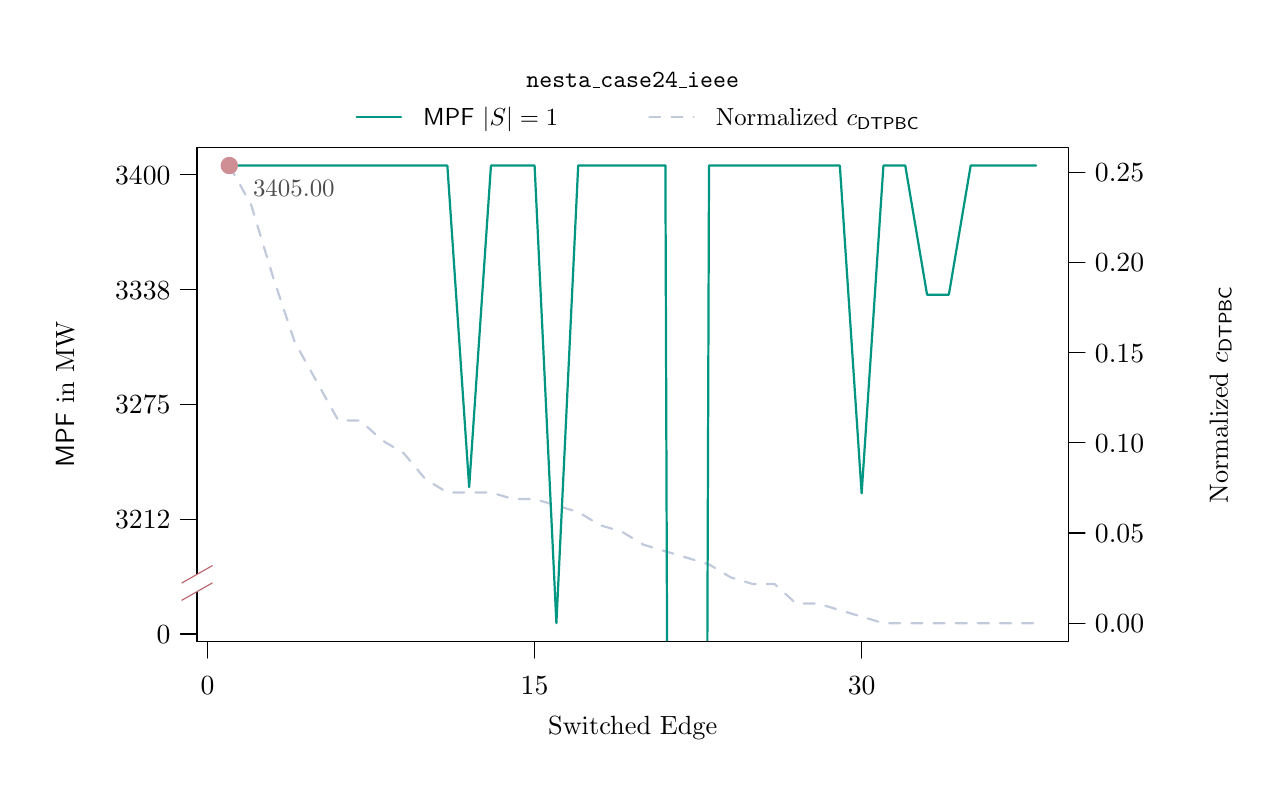
\begin{tikzpicture}[x=1pt,y=1pt]
\definecolor{fillColor}{RGB}{255,255,255}
\path[use as bounding box,fill=fillColor,fill opacity=0.00] (0,0) rectangle (440.85,271.01);
\begin{scope}
\path[clip] (  0.00,  0.00) rectangle (440.85,271.01);
\definecolor{drawColor}{RGB}{193,202,220}

\path[draw=drawColor,line width= 0.8pt,dash pattern=on 4pt off 4pt ,line join=round,line cap=round] ( 72.86,221.20) --
	( 80.74,207.02) --
	( 88.62,181.03) --
	( 96.50,157.41) --
	(104.38,143.23) --
	(112.26,129.06) --
	(120.14,129.06) --
	(128.01,121.97) --
	(135.89,117.24) --
	(143.77,107.79) --
	(151.65,103.07) --
	(159.53,103.07) --
	(167.41,103.07) --
	(175.29,100.70) --
	(183.17,100.70) --
	(191.05, 98.34) --
	(198.93, 95.98) --
	(206.80, 91.25) --
	(214.68, 88.89) --
	(222.56, 84.17) --
	(230.44, 81.80) --
	(238.32, 79.44) --
	(246.20, 77.08) --
	(254.08, 72.35) --
	(261.96, 69.99) --
	(269.84, 69.99) --
	(277.72, 62.90) --
	(285.60, 62.90) --
	(293.47, 60.54) --
	(301.35, 58.18) --
	(309.23, 55.82) --
	(317.11, 55.82) --
	(324.99, 55.82) --
	(332.87, 55.82) --
	(340.75, 55.82) --
	(348.63, 55.82) --
	(356.51, 55.82) --
	(364.39, 55.82);
\end{scope}
\begin{scope}
\path[clip] (  0.00,  0.00) rectangle (440.85,271.01);
\definecolor{drawColor}{RGB}{0,0,0}

\path[draw=drawColor,line width= 0.4pt,line join=round,line cap=round] ( 61.20, 49.20) --
	(376.05, 49.20) --
	(376.05,227.81) --
	( 61.20,227.81) --
	( 61.20, 49.20);
\end{scope}
\begin{scope}
\path[clip] (  0.00,  0.00) rectangle (440.85,271.01);
\definecolor{drawColor}{RGB}{0,0,0}

\path[draw=drawColor,line width= 0.4pt,line join=round,line cap=round] (376.05, 55.82) -- (376.05,218.83);

\path[draw=drawColor,line width= 0.4pt,line join=round,line cap=round] (376.05, 55.82) -- (382.05, 55.82);

\path[draw=drawColor,line width= 0.4pt,line join=round,line cap=round] (376.05, 88.42) -- (382.05, 88.42);

\path[draw=drawColor,line width= 0.4pt,line join=round,line cap=round] (376.05,121.02) -- (382.05,121.02);

\path[draw=drawColor,line width= 0.4pt,line join=round,line cap=round] (376.05,153.63) -- (382.05,153.63);

\path[draw=drawColor,line width= 0.4pt,line join=round,line cap=round] (376.05,186.23) -- (382.05,186.23);

\path[draw=drawColor,line width= 0.4pt,line join=round,line cap=round] (376.05,218.83) -- (382.05,218.83);

\node[text=drawColor,anchor=base west,inner sep=0pt, outer sep=0pt, scale=  1.00] at (385.65, 52.37) {0.00};

\node[text=drawColor,anchor=base west,inner sep=0pt, outer sep=0pt, scale=  1.00] at (385.65, 84.98) {0.05};

\node[text=drawColor,anchor=base west,inner sep=0pt, outer sep=0pt, scale=  1.00] at (385.65,117.58) {0.10};

\node[text=drawColor,anchor=base west,inner sep=0pt, outer sep=0pt, scale=  1.00] at (385.65,150.18) {0.15};

\node[text=drawColor,anchor=base west,inner sep=0pt, outer sep=0pt, scale=  1.00] at (385.65,182.79) {0.20};

\node[text=drawColor,anchor=base west,inner sep=0pt, outer sep=0pt, scale=  1.00] at (385.65,215.39) {0.25};
\end{scope}
\begin{scope}
\path[clip] (  0.00,  0.00) rectangle (440.85,271.01);
\definecolor{drawColor}{RGB}{0,150,130}

\path[draw=drawColor,line width= 0.8pt,line join=round,line cap=round] (118.89,238.60) -- (134.91,238.60);
\definecolor{drawColor}{RGB}{193,202,220}

\path[draw=drawColor,line width= 0.8pt,dash pattern=on 4pt off 4pt ,line join=round,line cap=round] (224.63,238.60) -- (240.65,238.60);
\definecolor{drawColor}{RGB}{0,0,0}

\node[text=drawColor,anchor=base,inner sep=0pt, outer sep=0pt, scale=  0.89] at (218.62,249.28) {\texttt{nesta\_case24\_ieee}};

\node[text=drawColor,anchor=base west,inner sep=0pt, outer sep=0pt, scale=  0.89] at (142.92,235.54) {$\mathsf{MPF}~|S|=1$};

\node[text=drawColor,anchor=base west,inner sep=0pt, outer sep=0pt, scale=  0.89] at (248.66,235.54) {Normalized~$c_\mathsf{DTPBC}$};
\end{scope}
\begin{scope}
\path[clip] (  0.00,  0.00) rectangle (440.85,271.01);
\definecolor{drawColor}{RGB}{0,0,0}

\path[draw=drawColor,line width= 0.4pt,line join=round,line cap=round] ( 61.20, 51.91) -- ( 61.20,217.88);

\path[draw=drawColor,line width= 0.4pt,line join=round,line cap=round] ( 61.20, 51.91) -- ( 55.20, 51.91);

\path[draw=drawColor,line width= 0.4pt,line join=round,line cap=round] ( 61.20, 93.40) -- ( 55.20, 93.40);

\path[draw=drawColor,line width= 0.4pt,line join=round,line cap=round] ( 61.20,134.89) -- ( 55.20,134.89);

\path[draw=drawColor,line width= 0.4pt,line join=round,line cap=round] ( 61.20,176.39) -- ( 55.20,176.39);

\path[draw=drawColor,line width= 0.4pt,line join=round,line cap=round] ( 61.20,217.88) -- ( 55.20,217.88);

\node[text=drawColor,anchor=base east,inner sep=0pt, outer sep=0pt, scale=  1.00] at ( 51.60, 48.47) {0};

\node[text=drawColor,anchor=base east,inner sep=0pt, outer sep=0pt, scale=  1.00] at ( 51.60, 89.96) {3212};

\node[text=drawColor,anchor=base east,inner sep=0pt, outer sep=0pt, scale=  1.00] at ( 51.60,131.45) {3275};

\node[text=drawColor,anchor=base east,inner sep=0pt, outer sep=0pt, scale=  1.00] at ( 51.60,172.94) {3338};

\node[text=drawColor,anchor=base east,inner sep=0pt, outer sep=0pt, scale=  1.00] at ( 51.60,214.43) {3400};
\end{scope}
\begin{scope}
\path[clip] (  0.00,  0.00) rectangle (440.85,271.01);
\definecolor{drawColor}{RGB}{255,255,255}
\definecolor{fillColor}{RGB}{255,255,255}

\path[draw=drawColor,line width= 0.4pt,line join=round,line cap=round,fill=fillColor] ( 55.69, 67.23) rectangle ( 66.71, 73.48);
\definecolor{drawColor}{RGB}{188,97,104}

\path[draw=drawColor,line width= 0.4pt,line join=round,line cap=round] ( 55.69, 64.10) -- ( 66.71, 70.35);

\path[draw=drawColor,line width= 0.4pt,line join=round,line cap=round] ( 55.69, 70.35) -- ( 66.71, 76.60);
\end{scope}
\begin{scope}
\path[clip] ( 61.20, 49.20) rectangle (376.05,227.81);
\definecolor{drawColor}{RGB}{0,150,130}

\path[draw=drawColor,line width= 0.8pt,line join=round,line cap=round] ( 72.86,221.20) --
	( 80.74,221.20) --
	( 88.62,221.20) --
	( 96.50,221.20) --
	(104.38,221.20) --
	(112.26,221.20) --
	(120.14,221.20) --
	(128.01,221.20) --
	(135.89,221.20) --
	(143.77,221.20) --
	(151.65,221.20) --
	(159.53,105.02) --
	(167.41,221.20) --
	(175.29,221.20) --
	(183.17,221.20) --
	(191.05, 55.82) --
	(198.93,221.20) --
	(206.80,221.20) --
	(214.68,221.20) --
	(222.56,221.20) --
	(230.44,221.20) --
	(231.21,  0.00);

\path[draw=drawColor,line width= 0.8pt,line join=round,line cap=round] (245.43,  0.00) --
	(246.20,221.20) --
	(254.08,221.20) --
	(261.96,221.20) --
	(269.84,221.20) --
	(277.72,221.20) --
	(285.60,221.20) --
	(293.47,221.20) --
	(301.35,102.74) --
	(309.23,221.20) --
	(317.11,221.20) --
	(324.99,174.53) --
	(332.87,174.53) --
	(340.75,221.20) --
	(348.63,221.20) --
	(356.51,221.20) --
	(364.39,221.20);
\end{scope}
\begin{scope}
\path[clip] ( 61.20, 49.20) rectangle (376.05,227.81);
\definecolor{fillColor}{RGB}{207,142,147}

\path[fill=fillColor] ( 72.86,221.20) circle (  3.15);
\end{scope}
\begin{scope}
\path[clip] ( 61.20, 49.20) rectangle (376.05,227.81);
\definecolor{drawColor}{gray}{0.30}

\node[text=drawColor,anchor=base,inner sep=0pt, outer sep=0pt, scale=  0.90] at ( 96.18,210.04) {3405.00};
\end{scope}
\begin{scope}
\path[clip] (  0.00,  0.00) rectangle (440.85,271.01);
\definecolor{drawColor}{RGB}{0,0,0}

\path[draw=drawColor,line width= 0.4pt,line join=round,line cap=round] ( 64.98, 49.20) -- (301.35, 49.20);

\path[draw=drawColor,line width= 0.4pt,line join=round,line cap=round] ( 64.98, 49.20) -- ( 64.98, 43.20);

\path[draw=drawColor,line width= 0.4pt,line join=round,line cap=round] (183.17, 49.20) -- (183.17, 43.20);

\path[draw=drawColor,line width= 0.4pt,line join=round,line cap=round] (301.35, 49.20) -- (301.35, 43.20);

\node[text=drawColor,anchor=base,inner sep=0pt, outer sep=0pt, scale=  1.00] at ( 64.98, 30.00) {0};

\node[text=drawColor,anchor=base,inner sep=0pt, outer sep=0pt, scale=  1.00] at (183.17, 30.00) {15};

\node[text=drawColor,anchor=base,inner sep=0pt, outer sep=0pt, scale=  1.00] at (301.35, 30.00) {30};

\node[text=drawColor,anchor=base,inner sep=0pt, outer sep=0pt, scale=  0.95] at (218.62, 15.60) {Switched Edge};

\node[text=drawColor,rotate= 90.00,anchor=base,inner sep=0pt, outer sep=0pt, scale=  0.95] at ( 16.80,138.51) {$\mathsf{MPF}$ in~$\mathrm{MW}$};

\node[text=drawColor,rotate= 90.00,anchor=base,inner sep=0pt, outer sep=0pt, scale=  0.95] at (433.65,138.51) {Normalized~$c_\mathsf{DTPBC}$};
\end{scope}
\end{tikzpicture}
